\documentclass[tikz,border=10pt]{standalone}

\usepackage{xcolor}
\usetikzlibrary{
    arrows.meta,
    positioning,
    fit,
    backgrounds,
    shapes.geometric
}

\begin{document}

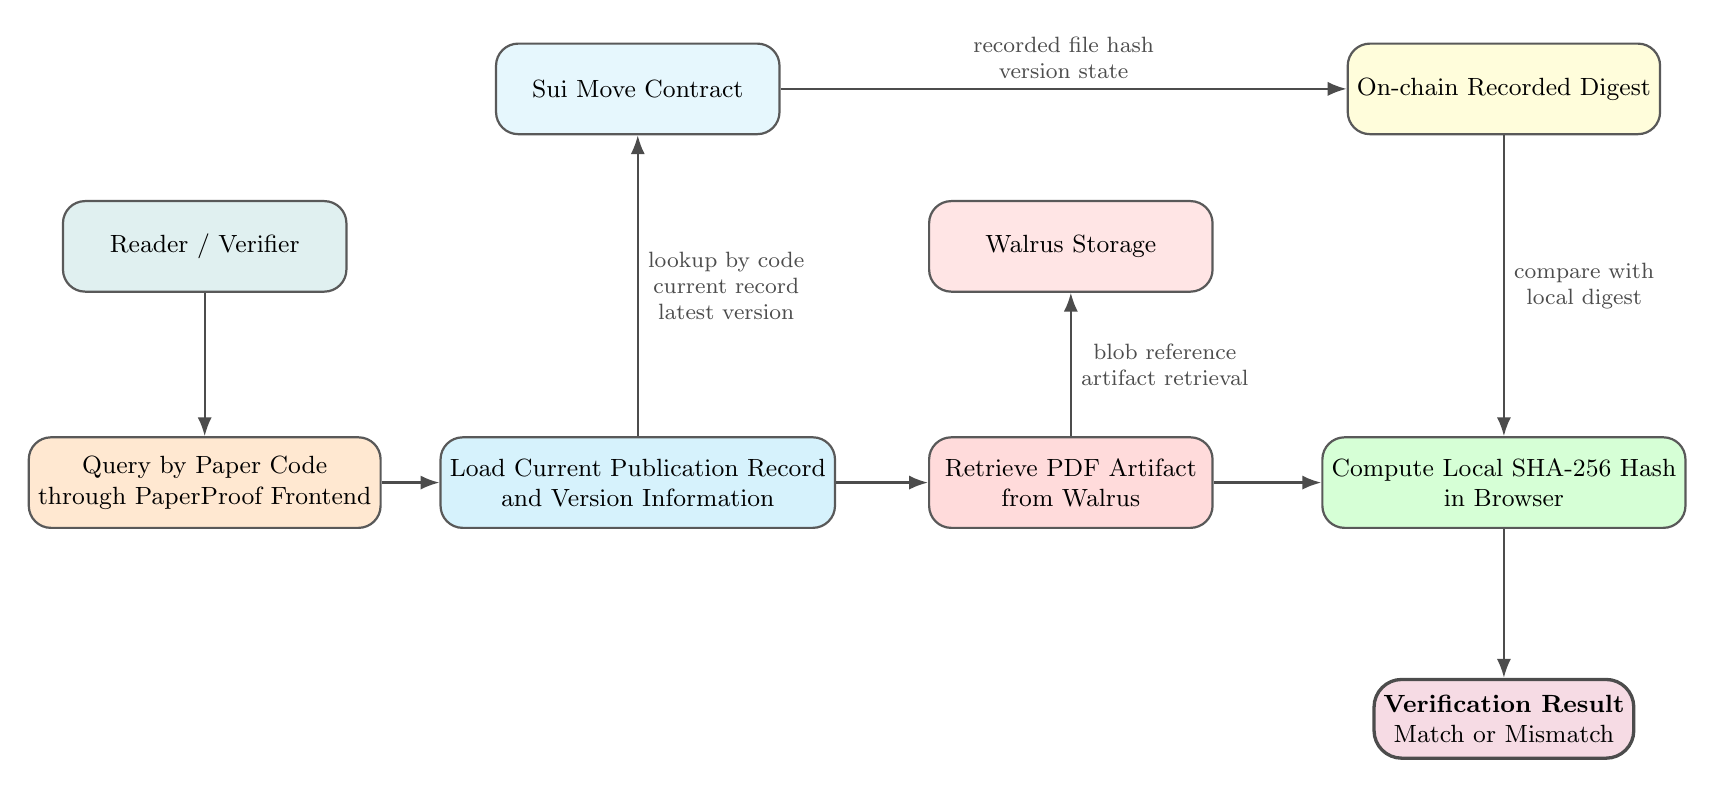
\begin{tikzpicture}[
    font=\small,
    box/.style={
        rectangle,
        rounded corners=8pt,
        draw=black!65,
        thick,
        align=center,
        minimum width=3.6cm,
        minimum height=1.15cm,
        fill=white
    },
    statebox/.style={
        rectangle,
        rounded corners=10pt,
        draw=black!70,
        very thick,
        align=center,
        minimum width=3.0cm,
        minimum height=1.0cm,
        fill=blue!10
    },
    arrow/.style={
        -{Latex[length=2.4mm,width=1.8mm]},
        thick,
        draw=black!70
    },
    note/.style={
        font=\footnotesize,
        align=center,
        text=black!70
    }
]

% =========================================================
% Main verification flow
% =========================================================
\node[box, fill=teal!12] (user) at (5.0,3)
{Reader / Verifier};

\node[box, fill=orange!18] (query) at (5.0,0)
{Query by Paper Code\\through PaperProof Frontend};

\node[box, fill=cyan!16] (record) at (10.5,0)
{Load Current Publication Record\\and Version Information};

\node[box, fill=red!14] (artifact) at (16.0,0)
{Retrieve PDF Artifact\\from Walrus};

\node[box, fill=green!16] (hashlocal) at (21.5,0)
{Compute Local SHA-256 Hash\\in Browser};

\node[statebox, fill=purple!14] (verify) at (21.5,-3)
{\textbf{Verification Result}\\Match or Mismatch};

% =========================================================
% Supporting references
% =========================================================
\node[box, fill=cyan!10] (sui) at (10.5,5.0)
{Sui Move Contract};

\node[box, fill=red!10] (walrus) at (16.0,3.0)
{Walrus Storage};

\node[box, fill=yellow!14] (digest) at (21.5,5.0)
{On-chain Recorded Digest};

% =========================================================
% Main arrows
% =========================================================
\draw[arrow] (user) -- (query);
\draw[arrow] (query) -- (record);
\draw[arrow] (record) -- (artifact);
\draw[arrow] (artifact) -- (hashlocal);
\draw[arrow] (hashlocal) -- (verify);

% =========================================================
% System interaction arrows
% =========================================================
\draw[arrow] (record) -- node[right, note] {lookup by code\\current record\\latest version} (sui);

\draw[arrow] (artifact) -- node[right, note] {blob reference\\artifact retrieval} (walrus);

\draw[arrow] (sui) -- node[above, note] {recorded file hash\\version state} (digest);

\draw[arrow] (digest) -- node[right, note] {compare with\\local digest} (hashlocal);

\end{tikzpicture}

\end{document}
